\documentclass[]{article}
\usepackage{lmodern}
\usepackage{amssymb,amsmath}
\usepackage{ifxetex,ifluatex}
\usepackage{fixltx2e} % provides \textsubscript
\ifnum 0\ifxetex 1\fi\ifluatex 1\fi=0 % if pdftex
  \usepackage[T1]{fontenc}
  \usepackage[utf8]{inputenc}
\else % if luatex or xelatex
  \ifxetex
    \usepackage{mathspec}
  \else
    \usepackage{fontspec}
  \fi
  \defaultfontfeatures{Ligatures=TeX,Scale=MatchLowercase}
\fi
% use upquote if available, for straight quotes in verbatim environments
\IfFileExists{upquote.sty}{\usepackage{upquote}}{}
% use microtype if available
\IfFileExists{microtype.sty}{%
\usepackage{microtype}
\UseMicrotypeSet[protrusion]{basicmath} % disable protrusion for tt fonts
}{}
\usepackage[margin=1in]{geometry}
\usepackage{hyperref}
\hypersetup{unicode=true,
            pdftitle={R Notebook},
            pdfborder={0 0 0},
            breaklinks=true}
\urlstyle{same}  % don't use monospace font for urls
\usepackage{color}
\usepackage{fancyvrb}
\newcommand{\VerbBar}{|}
\newcommand{\VERB}{\Verb[commandchars=\\\{\}]}
\DefineVerbatimEnvironment{Highlighting}{Verbatim}{commandchars=\\\{\}}
% Add ',fontsize=\small' for more characters per line
\newenvironment{Shaded}{}{}
\newcommand{\KeywordTok}[1]{\textcolor[rgb]{0.00,0.44,0.13}{\textbf{{#1}}}}
\newcommand{\DataTypeTok}[1]{\textcolor[rgb]{0.56,0.13,0.00}{{#1}}}
\newcommand{\DecValTok}[1]{\textcolor[rgb]{0.25,0.63,0.44}{{#1}}}
\newcommand{\BaseNTok}[1]{\textcolor[rgb]{0.25,0.63,0.44}{{#1}}}
\newcommand{\FloatTok}[1]{\textcolor[rgb]{0.25,0.63,0.44}{{#1}}}
\newcommand{\ConstantTok}[1]{\textcolor[rgb]{0.53,0.00,0.00}{{#1}}}
\newcommand{\CharTok}[1]{\textcolor[rgb]{0.25,0.44,0.63}{{#1}}}
\newcommand{\SpecialCharTok}[1]{\textcolor[rgb]{0.25,0.44,0.63}{{#1}}}
\newcommand{\StringTok}[1]{\textcolor[rgb]{0.25,0.44,0.63}{{#1}}}
\newcommand{\VerbatimStringTok}[1]{\textcolor[rgb]{0.25,0.44,0.63}{{#1}}}
\newcommand{\SpecialStringTok}[1]{\textcolor[rgb]{0.73,0.40,0.53}{{#1}}}
\newcommand{\ImportTok}[1]{{#1}}
\newcommand{\CommentTok}[1]{\textcolor[rgb]{0.38,0.63,0.69}{\textit{{#1}}}}
\newcommand{\DocumentationTok}[1]{\textcolor[rgb]{0.73,0.13,0.13}{\textit{{#1}}}}
\newcommand{\AnnotationTok}[1]{\textcolor[rgb]{0.38,0.63,0.69}{\textbf{\textit{{#1}}}}}
\newcommand{\CommentVarTok}[1]{\textcolor[rgb]{0.38,0.63,0.69}{\textbf{\textit{{#1}}}}}
\newcommand{\OtherTok}[1]{\textcolor[rgb]{0.00,0.44,0.13}{{#1}}}
\newcommand{\FunctionTok}[1]{\textcolor[rgb]{0.02,0.16,0.49}{{#1}}}
\newcommand{\VariableTok}[1]{\textcolor[rgb]{0.10,0.09,0.49}{{#1}}}
\newcommand{\ControlFlowTok}[1]{\textcolor[rgb]{0.00,0.44,0.13}{\textbf{{#1}}}}
\newcommand{\OperatorTok}[1]{\textcolor[rgb]{0.40,0.40,0.40}{{#1}}}
\newcommand{\BuiltInTok}[1]{{#1}}
\newcommand{\ExtensionTok}[1]{{#1}}
\newcommand{\PreprocessorTok}[1]{\textcolor[rgb]{0.74,0.48,0.00}{{#1}}}
\newcommand{\AttributeTok}[1]{\textcolor[rgb]{0.49,0.56,0.16}{{#1}}}
\newcommand{\RegionMarkerTok}[1]{{#1}}
\newcommand{\InformationTok}[1]{\textcolor[rgb]{0.38,0.63,0.69}{\textbf{\textit{{#1}}}}}
\newcommand{\WarningTok}[1]{\textcolor[rgb]{0.38,0.63,0.69}{\textbf{\textit{{#1}}}}}
\newcommand{\AlertTok}[1]{\textcolor[rgb]{1.00,0.00,0.00}{\textbf{{#1}}}}
\newcommand{\ErrorTok}[1]{\textcolor[rgb]{1.00,0.00,0.00}{\textbf{{#1}}}}
\newcommand{\NormalTok}[1]{{#1}}
\usepackage{graphicx,grffile}
\makeatletter
\def\maxwidth{\ifdim\Gin@nat@width>\linewidth\linewidth\else\Gin@nat@width\fi}
\def\maxheight{\ifdim\Gin@nat@height>\textheight\textheight\else\Gin@nat@height\fi}
\makeatother
% Scale images if necessary, so that they will not overflow the page
% margins by default, and it is still possible to overwrite the defaults
% using explicit options in \includegraphics[width, height, ...]{}
\setkeys{Gin}{width=\maxwidth,height=\maxheight,keepaspectratio}
\IfFileExists{parskip.sty}{%
\usepackage{parskip}
}{% else
\setlength{\parindent}{0pt}
\setlength{\parskip}{6pt plus 2pt minus 1pt}
}
\setlength{\emergencystretch}{3em}  % prevent overfull lines
\providecommand{\tightlist}{%
  \setlength{\itemsep}{0pt}\setlength{\parskip}{0pt}}
\setcounter{secnumdepth}{0}
% Redefines (sub)paragraphs to behave more like sections
\ifx\paragraph\undefined\else
\let\oldparagraph\paragraph
\renewcommand{\paragraph}[1]{\oldparagraph{#1}\mbox{}}
\fi
\ifx\subparagraph\undefined\else
\let\oldsubparagraph\subparagraph
\renewcommand{\subparagraph}[1]{\oldsubparagraph{#1}\mbox{}}
\fi

%%% Use protect on footnotes to avoid problems with footnotes in titles
\let\rmarkdownfootnote\footnote%
\def\footnote{\protect\rmarkdownfootnote}

%%% Change title format to be more compact
\usepackage{titling}

% Create subtitle command for use in maketitle
\newcommand{\subtitle}[1]{
  \posttitle{
    \begin{center}\large#1\end{center}
    }
}

\setlength{\droptitle}{-2em}
  \title{R Notebook}
  \pretitle{\vspace{\droptitle}\centering\huge}
  \posttitle{\par}
  \author{}
  \preauthor{}\postauthor{}
  \date{}
  \predate{}\postdate{}


\begin{document}
\maketitle

Analysis of equilibrium resonse to power law scaling behaviors,
single-consumer resource case.

\begin{Shaded}
\begin{Highlighting}[]
\KeywordTok{library}\NormalTok{(tidyverse)}
\end{Highlighting}
\end{Shaded}

\begin{Shaded}
\begin{Highlighting}[]
\NormalTok{n.dat <-}\StringTok{ }\KeywordTok{read_csv}\NormalTok{(}\StringTok{'socio-eco-nw equilibrium-pop-table.csv'}\NormalTok{, }\DataTypeTok{skip =} \DecValTok{6}\NormalTok{) %>%}
\StringTok{  }\KeywordTok{select}\NormalTok{(alpha, beta, }\DataTypeTok{pop =} \DecValTok{12}\NormalTok{)}
\end{Highlighting}
\end{Shaded}

\begin{verbatim}
## Parsed with column specification:
## cols(
##   `[run number]` = col_integer(),
##   r = col_double(),
##   `harvest-rate` = col_double(),
##   alpha = col_double(),
##   k = col_integer(),
##   `link-prob` = col_integer(),
##   beta = col_double(),
##   `conversion-efficiency` = col_double(),
##   `death-rate` = col_double(),
##   n = col_integer(),
##   `[step]` = col_integer(),
##   `[size] of social-system 0` = col_double()
## )
\end{verbatim}

\begin{Shaded}
\begin{Highlighting}[]
\NormalTok{x.dat <-}\StringTok{ }\KeywordTok{read_csv}\NormalTok{(}\StringTok{'socio-eco-nw equilibrium-bio-table.csv'}\NormalTok{, }\DataTypeTok{skip =} \DecValTok{6}\NormalTok{) %>%}
\StringTok{  }\KeywordTok{select}\NormalTok{(alpha, beta, }\DataTypeTok{biomass =} \DecValTok{12}\NormalTok{)}
\end{Highlighting}
\end{Shaded}

\begin{verbatim}
## Parsed with column specification:
## cols(
##   `[run number]` = col_integer(),
##   r = col_double(),
##   `harvest-rate` = col_double(),
##   alpha = col_double(),
##   k = col_integer(),
##   `link-prob` = col_integer(),
##   beta = col_double(),
##   `conversion-efficiency` = col_double(),
##   `death-rate` = col_double(),
##   n = col_integer(),
##   `[step]` = col_integer(),
##   `[size] of ecosystem 1` = col_double()
## )
\end{verbatim}

\begin{Shaded}
\begin{Highlighting}[]
\KeywordTok{ggplot}\NormalTok{(n.dat, }\KeywordTok{aes}\NormalTok{(alpha, beta, }\DataTypeTok{fill =} \NormalTok{pop /}\StringTok{ }\DecValTok{60000}\NormalTok{)) +}
\StringTok{  }\KeywordTok{geom_raster}\NormalTok{(}\DataTypeTok{interpolate =} \NormalTok{T) +}
\StringTok{  }\KeywordTok{labs}\NormalTok{(}\DataTypeTok{title =} \StringTok{'Equilibrium population size'}\NormalTok{, }\DataTypeTok{subtitle =} \StringTok{'Sensitivity to power-law scaling'}\NormalTok{, }\DataTypeTok{x =} \StringTok{'Alpha'}\NormalTok{, }\DataTypeTok{y =} \StringTok{'Beta'}\NormalTok{) +}
\StringTok{  }\KeywordTok{scale_fill_distiller}\NormalTok{(}\DataTypeTok{name =} \StringTok{'Normalized }\CharTok{\textbackslash{}n}\StringTok{population'}\NormalTok{, }\DataTypeTok{palette =} \StringTok{'Spectral'}\NormalTok{) +}
\StringTok{  }\KeywordTok{coord_equal}\NormalTok{() +}
\StringTok{  }\KeywordTok{theme_minimal}\NormalTok{()}
\end{Highlighting}
\end{Shaded}

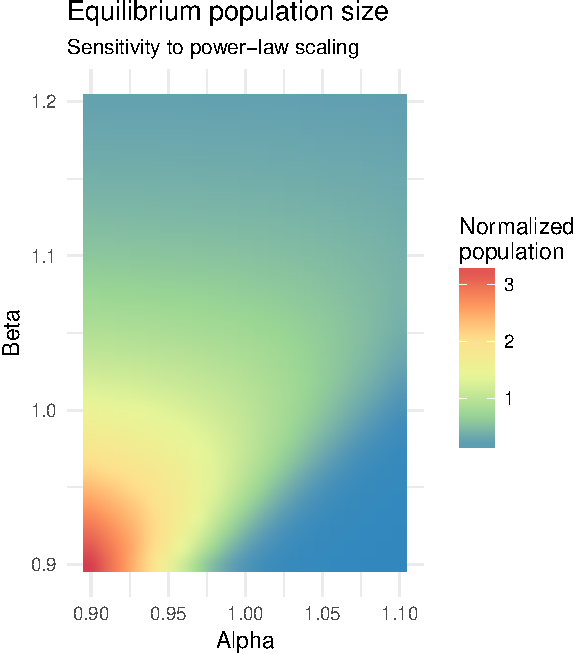
\includegraphics{eq_pop_files/figure-latex/unnamed-chunk-3-1.pdf}

\begin{Shaded}
\begin{Highlighting}[]
\NormalTok{n.dat %>%}\StringTok{ }\KeywordTok{filter}\NormalTok{(alpha ==}\StringTok{ }\DecValTok{1} \NormalTok{&}\StringTok{ }\NormalTok{beta ==}\StringTok{ }\DecValTok{1}\NormalTok{)}
\end{Highlighting}
\end{Shaded}

\begin{verbatim}
## # A tibble: 1 × 3
##   alpha  beta   pop
##   <dbl> <dbl> <dbl>
## 1     1     1 60000
\end{verbatim}

\begin{Shaded}
\begin{Highlighting}[]
\NormalTok{x.dat %>%}\StringTok{ }\KeywordTok{filter}\NormalTok{(alpha ==}\StringTok{ }\DecValTok{1} \NormalTok{&}\StringTok{ }\NormalTok{beta ==}\StringTok{ }\DecValTok{1}\NormalTok{)}
\end{Highlighting}
\end{Shaded}

\begin{verbatim}
## # A tibble: 1 × 3
##   alpha  beta biomass
##   <dbl> <dbl>   <dbl>
## 1     1     1     0.4
\end{verbatim}

\begin{Shaded}
\begin{Highlighting}[]
\KeywordTok{ggplot}\NormalTok{(x.dat, }\KeywordTok{aes}\NormalTok{(alpha, beta, }\DataTypeTok{fill =} \NormalTok{biomass/.}\DecValTok{4}\NormalTok{)) +}
\StringTok{  }\KeywordTok{geom_raster}\NormalTok{(}\DataTypeTok{interpolate =} \NormalTok{T) +}
\StringTok{  }\KeywordTok{labs}\NormalTok{(}\DataTypeTok{title =} \StringTok{'Equilibrium population size'}\NormalTok{, }\DataTypeTok{subtitle =} \StringTok{'Sensitivity to power-law scaling'}\NormalTok{, }\DataTypeTok{x =} \StringTok{'Alpha'}\NormalTok{, }\DataTypeTok{y =} \StringTok{'Beta'}\NormalTok{) +}
\StringTok{  }\KeywordTok{scale_fill_distiller}\NormalTok{(}\DataTypeTok{name =} \StringTok{'Normalized }\CharTok{\textbackslash{}n}\StringTok{biomass'}\NormalTok{, }\DataTypeTok{palette =} \StringTok{'Spectral'}\NormalTok{) +}
\StringTok{  }\KeywordTok{coord_equal}\NormalTok{() +}
\StringTok{  }\KeywordTok{theme_minimal}\NormalTok{()}
\end{Highlighting}
\end{Shaded}

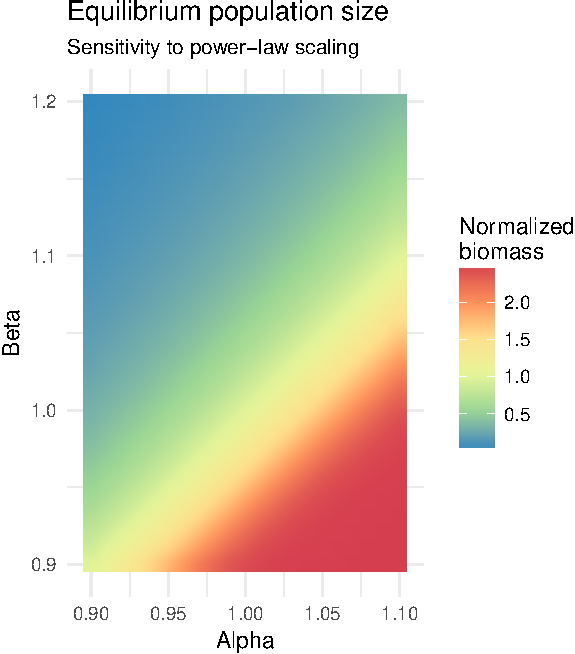
\includegraphics{eq_pop_files/figure-latex/unnamed-chunk-5-1.pdf}

\begin{Shaded}
\begin{Highlighting}[]
\KeywordTok{ggplot}\NormalTok{(n.dat, }\KeywordTok{aes}\NormalTok{(alpha, beta, }\DataTypeTok{fill =} \NormalTok{pop /}\StringTok{ }\DecValTok{60000}\NormalTok{)) +}
\StringTok{  }\KeywordTok{geom_raster}\NormalTok{(}\DataTypeTok{interpolate =} \NormalTok{T) +}
\StringTok{  }\KeywordTok{labs}\NormalTok{(}\DataTypeTok{title =} \StringTok{'Equilibrium sensitivity to power-law scaling'}\NormalTok{, }\DataTypeTok{subtitle =} \StringTok{'Consumer population'}\NormalTok{, }\DataTypeTok{x =} \StringTok{'Alpha'}\NormalTok{, }\DataTypeTok{y =} \StringTok{'Beta'}\NormalTok{) +}
\StringTok{  }\KeywordTok{scale_fill_distiller}\NormalTok{(}\DataTypeTok{name =} \StringTok{'Normalized }\CharTok{\textbackslash{}n}\StringTok{population'}\NormalTok{, }\DataTypeTok{palette =} \StringTok{'Spectral'}\NormalTok{, }\DataTypeTok{position =} \StringTok{'bottom'}\NormalTok{) +}
\StringTok{  }\KeywordTok{coord_equal}\NormalTok{() +}
\StringTok{  }\KeywordTok{theme_minimal}\NormalTok{()}

\KeywordTok{ggplot}\NormalTok{(x.dat, }\KeywordTok{aes}\NormalTok{(alpha, beta, }\DataTypeTok{fill =} \NormalTok{biomass/.}\DecValTok{4}\NormalTok{)) +}
\StringTok{  }\KeywordTok{geom_raster}\NormalTok{(}\DataTypeTok{interpolate =} \NormalTok{T) +}
\StringTok{  }\KeywordTok{labs}\NormalTok{(}\DataTypeTok{title =} \StringTok{''}\NormalTok{, }\DataTypeTok{subtitle =} \StringTok{'Resource biomass'}\NormalTok{, }\DataTypeTok{x =} \StringTok{'Alpha'}\NormalTok{, }\DataTypeTok{y =} \StringTok{'Beta'}\NormalTok{) +}
\StringTok{  }\KeywordTok{scale_fill_distiller}\NormalTok{(}\DataTypeTok{name =} \StringTok{'Normalized }\CharTok{\textbackslash{}n}\StringTok{biomass'}\NormalTok{, }\DataTypeTok{palette =} \StringTok{'Spectral'}\NormalTok{, }\DataTypeTok{position =} \StringTok{'bottom'}\NormalTok{) +}
\StringTok{  }\KeywordTok{coord_equal}\NormalTok{() +}
\StringTok{  }\KeywordTok{theme_minimal}\NormalTok{()}
\end{Highlighting}
\end{Shaded}

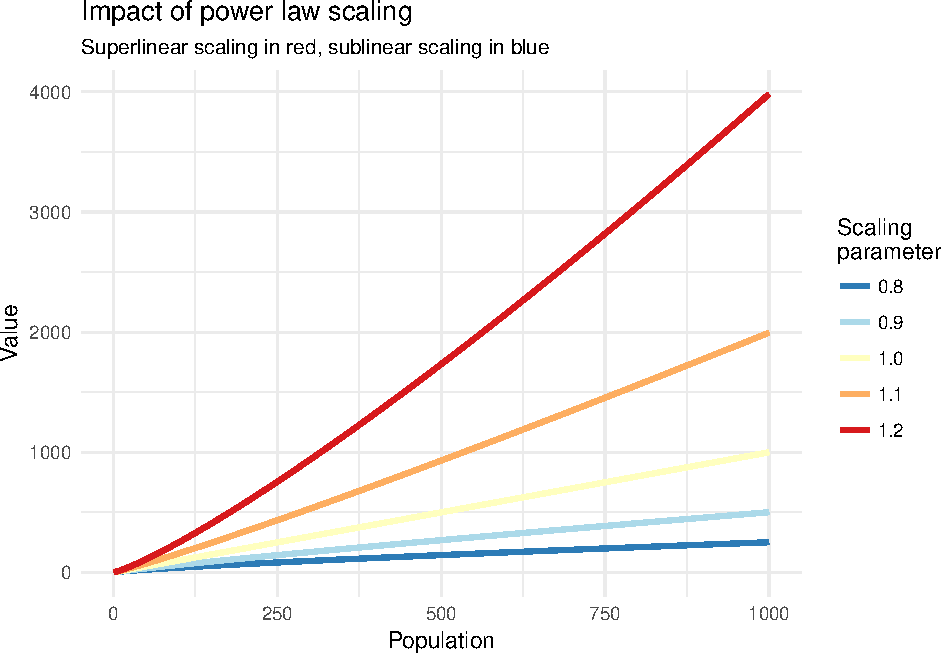
\includegraphics[width=1\linewidth]{eq_pop_files/figure-latex/unnamed-chunk-6-1}
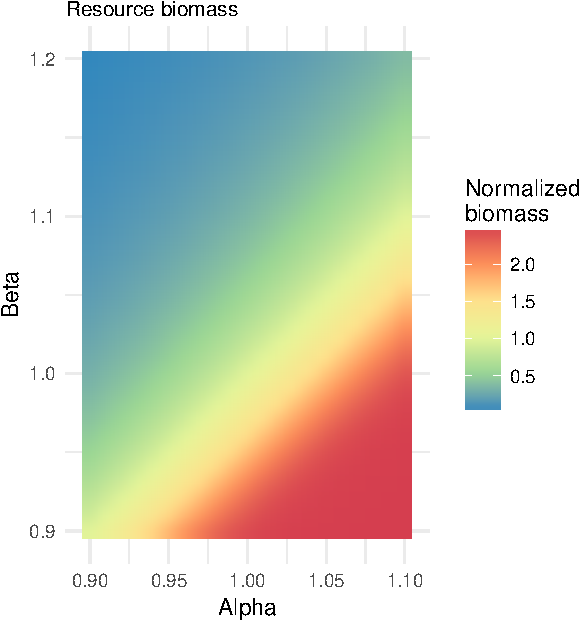
\includegraphics[width=1\linewidth]{eq_pop_files/figure-latex/unnamed-chunk-6-2}


\end{document}
